\documentclass[11pt]{article}

% Language setting
% Replace `english' with e.g. `spanish' to change the document language
\usepackage[english]{babel}

% Set page size and margins
% Replace `letterpaper' with`a4paper' for UK/EU standard size
\usepackage[a4paper,top=2cm,bottom=2cm,left=2cm,right=2cm,marginparwidth=1.75cm]{geometry}

% Useful packages
\usepackage{array}
\usepackage{amsmath}
\usepackage{graphicx}
\usepackage{tcolorbox}
\usepackage[colorlinks=true, allcolors=blue]{hyperref}
\usepackage{fancyhdr}
\usepackage{lastpage}
\usepackage{multirow}
\usepackage{indentfirst}
\usepackage[section]{placeins}

\makeatletter
\AtBeginDocument{%
  \expandafter\renewcommand\expandafter\subsubsection\expandafter{%
    \expandafter\@fb@secFB\subsubsection
  }%
}
\makeatother
\makeatletter
\AtBeginDocument{%
  \expandafter\renewcommand\expandafter\subsection\expandafter{%
    \expandafter\@fb@secFB\subsection
  }%
}
\makeatother


\begin{document}
\pagestyle{fancy}


%% ------------ Footer ------------ %%
\fancyhf{}
\renewcommand{\headrulewidth}{0pt}
\fancyfoot[RE,LO]{\textbf{Team 001}}  %CHANGE
\fancyfoot[LE,RO]{Page \thepage}
%% -------------------------------------- %%

%% ------------ HEADER COMMANDS ------------ %%
\newcolumntype{L}[1]{>{\raggedright\let\newline\\\arraybackslash\hspace{0pt}}m{#1}}
\newcolumntype{C}[1]{>{\centering\let\newline\\\arraybackslash\hspace{0pt}}m{#1}}
\newcolumntype{R}[1]{>{\raggedleft\let\newline\\\arraybackslash\hspace{0pt}}m{#1}}
%% ------------ HEADER ------------ %%
\noindent\begin{tabular}{L{3.5cm}C{9cm}R{3cm}}
   \includegraphics[width=3.5cm]{tecnico.png} &  & \huge DS 2021\\
   & & \\
   & \Huge \textbf{Data Science Project} & \\
   & &
\end{tabular}
%% -------------------------------------- %%

\begin{center}
    \begin{tabular}{ | c | l l c | }
     \hline
     \multirow{3}{*}{Team Nr. 001} & Student 1 & António Maria Rodrigues Venâncio\hspace{2cm} & IST-ID: 93689 \\ \cline{2-4}
     & Student 2 & Diogo Miguel Catarino Cabral & IST-ID: 93704 \\ \cline{2-4} 
     & Student 3 & Nelson Alexandre Geada Trindade & IST-ID: 93743 \\\hline    
    \end{tabular}
\end{center}

%\begin{tcolorbox} %Remove from final report
%The present document presents a template for the Data Science Project report. It specifies the mandatory format and suggests the structure to follow. Intermediate headings (non-numbered ones) are not mandatory since they occupy to much space, but their usage is encouraged. The report \textbf{cannot exceeds 15 pages} (excluding the appendix).
%All text with grey background shall be removed on the final report.
%\end{tcolorbox} %Remove from final report

\section{DATA PROFILING}
%\begin{tcolorbox} %Remove from final report
%May be used to describe any useful observation about the data, and that was used in the current project. An example is the use of any domain knowledge to process the data or evaluate the results.
%\end{tcolorbox} %Remove from final report
\fcolorbox{cyan}{cyan}{Dataset1} The first look at the dataset corresponding to traffic collisions in NYC throughout the year 2021 can already gives us relevant information on how the data should be prepared. First of all, there are many features present whose sole purpose is identification (i.e ID variables) which will not help us in the KDD process.

\fcolorbox{orange}{orange}{Dataset2} FALTA algo FALTA algo FALTA algo FALTA algo FALTA algo FALTA algo FALTA algo FALTA algo FALTA algo FALTA algo FALTA algo FALTA algo FALTA algo FALTA algo FALTA algo FALTA algo FALTA algo FALTA algo FALTA algo FALTA algo FALTA algo FALTA algo FALTA algo FALTA algo FALTA algo FALTA algo FALTA algo FALTA algo FALTA algo FALTA algo FALTA algo FALTA algo FALTA algo FALTA algo FALTA algo FALTA algo 

\subsection*{Data Dimensionality}
%\begin{tcolorbox} %Remove from final report
%Shall contain all relevant information and charts respecting to the data dimensionality perspective, such as the number of records and number of dimensions, 

%-->>and their impact on the following analysis.

%\end{tcolorbox} %Remove from final report
\fcolorbox{cyan}{cyan}{Dataset1} For NYC Collisions dataset, we have 45669 records and 21 variables, which have different types: 4 are Numeric, 1 Binary\footnote[1]{The Class Variable} and 16 Symbolic. Considering the number of Missing Values, we have 9 variables that have this issue, being PED\_LOCATION, CONTRIBUTING\_FACTOR\_2, CONTRIBUTING\_FACTOR\_1, and PED\_ACTION with the most missing values (around 39100 each).

\begin{figure*}[!htp]
    \begin{minipage}[!htp]{.33\textwidth}
        \centering
        \includegraphics[width=.95\linewidth]{imagens/dataProfiling/set1/records_variables.png}
        Set1 - Dimensionality
    \end{minipage}\hfill
    \begin{minipage}[!htp]{.33\textwidth}
        \centering
        \includegraphics[width=.95\linewidth]{imagens/dataProfiling/set1/variable_types.png}
        Set1 - Variables per type
    \end{minipage}\hfill
    \begin{minipage}[!htp]{.33\textwidth}
        \centering
        \includegraphics[width=.95\linewidth]{imagens/dataProfiling/set1/missing_values.png}
        Set1 - Missing Values
    \end{minipage}\hfill
\end{figure*}

\fcolorbox{orange}{orange}{Dataset2} For Air Quality dataset, we have 169273 records and 31 variables. From this variables: 27 are Numeric, 1 Binary\footnotemark[1] and 3 Symbolic. Considering the number of Missing Values, we have 24 variables with an average of 7750 missing values, and Field\_1 as 17062. 

\begin{figure*}[!htp]
    \begin{minipage}[!htp]{.33\textwidth}
        \centering
        \includegraphics[width=.95\linewidth]{imagens/dataProfiling/set2/records_variables.png}
        Set2 - Dimensionality
    \end{minipage}\hfill
    \begin{minipage}[!htp]{.33\textwidth}
        \centering
        \includegraphics[width=.95\linewidth]{imagens/dataProfiling/set2/variable_types.png}
        Set2 - Variables per type
    \end{minipage}\hfill
    \begin{minipage}[!htp]{.33\textwidth}
        \centering
        \includegraphics[width=.95\linewidth]{imagens/dataProfiling/set2/missing_values.png}
        Set2 - Missing Values
    \end{minipage}\hfill
\end{figure*}


\subsection*{Data Granularity}
%\begin{tcolorbox} %Remove from final report
%Shall contain all relevant information and charts respecting to the data granularity perspective, such as the impact of different granularities considered for each variable. Redundant or non-fundamental charts can be appended in Appendix. 
%\end{tcolorbox} %Remove from final report
\fcolorbox{cyan}{cyan}{Dataset1} ASDASDA

\fcolorbox{orange}{orange}{Dataset2} For dataset 2 we have several variables present that represent a normal distribution (approximately). Besides this fact, certain histograms pose possible indicators for the presence of outliers, in particular PM10\_Std, PM10\_Min, PM10\_Max, PM10\_Mean as well as many others. To conclude, if we look at "GbProv" histogram, it does not possess an adequate number of bins. If reduced to 10 bins, there may be a better way to acess a proper distribution.


\begin{figure*}[!htp]
    \begin{minipage}[!htp]{.50\textwidth}
        \centering
        \includegraphics[width=.95\linewidth]{imagens/dataProfiling/set1/histogram_numeric.png}
        Set1 - Granularity
    \end{minipage}\hfill
    \begin{minipage}[!htp]{.40\textwidth}
        \centering
        \includegraphics[width=.95\linewidth]{imagens/dataProfiling/set2/granularity_single.png}
        Set2 - Granularity
    \end{minipage}\hfill
\end{figure*}


\subsection*{Data Distribution}
%\begin{tcolorbox} %Remove from final report
%Shall contain all relevant information and charts respecting to the data distribution perspective, such as each variable distribution, type, domain and range. Redundant or non-fundamental charts can be appended in Appendix. 
%\end{tcolorbox} %Remove from final report
\fcolorbox{cyan}{cyan}{Dataset1}

\fcolorbox{orange}{orange}{Dataset2}

\subsection*{Data Sparsity}
\begin{tcolorbox} %Remove from final report
Shall contain all relevant information and charts respecting to the data sparsity perspective, such as domain coverage and correlation among variables. Redundant or non-fundamental charts can be appended in Appendix. 
\end{tcolorbox} %Remove from final report
\fcolorbox{cyan}{cyan}{Dataset1}

\fcolorbox{orange}{orange}{Dataset2}


\section{DATA PREPARATION}
%\begin{tcolorbox} %Remove from final report
%May be used to summarize any useful observation derived from data profiling to better understand the choices followed ahead. Can contain the preparation of date variables, but not the prediction variable.
%\end{tcolorbox} %Remove from final report
\fcolorbox{cyan}{cyan}{Dataset1}

\fcolorbox{orange}{orange}{Dataset2}
In the last section, we notice some odd aspects. For instance, the graph showed in the data dimensionality shows that we have 5 symbolic variables: "FID", "City\_EN", "Prov\_EN", "GbCity", "GbProv". The "City\_EN" and "Prov\_EN" where correct, they are symbolic values (They represent text). However the others aren't.
We also checked if there were negative values in all the numerical variables, in order to see if it made sense or not, but there aren't negative values in this stage.

When we took a glance in the "GbCity" variable, we saw that 65536 records were considered to be a string. In this records we come across that 152 records that contained a 's' instead of a number. In this cases, the first attempt was to treat them as missing values, but we gave a second look and realized that this no-numerical values followed a pattern in the variable "GbCity": \{3410,3411,'s',3413,3414\}. Since all followed that same pattern, we replaced the 's' with 3412, and applied the technique of converting all to float.

We took a look into the "FID" and "GbProv" variables, to check if there were no-numerical values, but all records are numerical and with the change of the variable "GbCity" to numerical, this variables became numerical as well.

\subsection*{Missing Value Imputation}
%\begin{tcolorbox} %Remove from final report
%Shall contain all relevant information and charts respecting to missing values imputation, such as the choices made and the impact of the different approaches on modeling results. Shall also clearly reveal the approach selected to proceed with the processing. 
%If not applied explain the reason for that, based on data characteristics.
%\end{tcolorbox} %Remove from final report
\fcolorbox{cyan}{cyan}{Dataset1}

\fcolorbox{orange}{orange}{Dataset2}
As you can see in the graph below, we have more than 9000 missing values in all variables, but not all of them are worth to keep. We discard the records that had $50\%$ of the variables missing, and discard all variables that have $90\%$ of missing values. The result of the first process can be verified by the figure x, and the second process didn't removed any variable. We used the mean term to threat numeric values, and the most frequent term to threat symbolic and binary values. The result can be seen in the figure X. We chose to do this, because in our tests, the result of the //TODO

\subsection*{Dummification and other transformations}
%\begin{tcolorbox} %Remove from final report
%Shall contain all relevant information respecting to the transformation of variables, including dummification,. The list of variables under each one of the transformations shall be presented. 
%If not applied explain the reason for that, based on data characteristics.
%\end{tcolorbox} %Remove from final report
\fcolorbox{cyan}{cyan}{Dataset1}

\fcolorbox{orange}{orange}{Dataset2}
For the second dataset, we didn't do dummification. We made this decision, because it would transform the dataset from 31 variables into X variables, and in terms of time it would take longer to train a model. Instead, we acknowledge that we had small\footnote{\label{small_variation}comparing with the large dataset} variations in the variable "IDK" (unique records) and in the variable "IDK" (unique records). With this in mind, we mapped ids to the "" column, and change the values to this ids (Same process to "" column).


\subsection*{Outliers Imputation}
\begin{tcolorbox} %Remove from final report
Shall contain all relevant information and charts respecting to outliers imputation, such as the choices made and the impact of the different approaches on modeling results. Shall also clearly reveal the approach selected to proceed with the processing. 
If not applied explain the reason for that, based on data characteristics.
\end{tcolorbox} %Remove from final report
\fcolorbox{cyan}{cyan}{Dataset1}

\fcolorbox{orange}{orange}{Dataset2}



\subsection*{Scaling}
\begin{tcolorbox} %Remove from final report
Shall contain all relevant information and charts respecting to scaling transformation, such as the choices made and the impact of the different approaches on modeling results. Shall also clearly reveal the approach selected to proceed with the processing. 
If not applied explain the reason for that, based on data characteristics.
\end{tcolorbox} %Remove from final report
\fcolorbox{cyan}{cyan}{Dataset1}

\fcolorbox{orange}{orange}{Dataset2}

\subsection*{Balancing}
\begin{tcolorbox} %Remove from final report
Shall contain all relevant information and charts respecting to balancing transformation, such as the choices made and the impact of the different approaches on modeling results. Shall also clearly reveal the approach selected to proceed with the processing. 
If not applied explain the reason for that, based on data characteristics.
\end{tcolorbox} %Remove from final report
\fcolorbox{cyan}{cyan}{Dataset1}

\fcolorbox{orange}{orange}{Dataset2}

\subsection{Feature Engineering}
\subsubsection*{Feature Selection}
\begin{tcolorbox} %Remove from final report
Shall contain all relevant information and charts respecting to feature selection based on filtering out redundant variables. The different choices and their impact on the modeling results shall be presented and explained. Should also clearly reveal the approach selected to proceed with the processing. 
All explanations shall be based on data characteristics.
\end{tcolorbox} %Remove from final report
\begin{tcolorbox} %Remove from final report
Shall contain all relevant information and charts respecting to feature selection based on filtering out irrelevant variables. The different choices and their impact on the modeling results shall be presented and explained. Should also clearly reveal the approach selected to proceed with the processing. 
All explanations shall be based on data characteristics.
\end{tcolorbox} %Remove from final report
\fcolorbox{cyan}{cyan}{Dataset1}

\fcolorbox{orange}{orange}{Dataset2}

\subsubsection*{Feature Extraction}
\begin{tcolorbox} %Remove from final report
Shall contain all relevant information and charts respecting to feature extraction, in particular PCA. The different choices and their impact on the modeling results shall be presented and explained. 
\end{tcolorbox} %Remove from final report
\fcolorbox{cyan}{cyan}{Dataset1}

\fcolorbox{orange}{orange}{Dataset2}

\subsubsection*{Feature Generation}
\begin{tcolorbox} %Remove from final report
Shall contain all relevant information and charts respecting to feature generation. The different choices and their impact on the modeling results shall be presented and explained. Shall list all variables generated and the formula used to derive them. 
\end{tcolorbox} %Remove from final report
\fcolorbox{cyan}{cyan}{Dataset1}

\fcolorbox{orange}{orange}{Dataset2}

\section{CLASSIFICATION}
\begin{tcolorbox} %Remove from final report
Shall be used to summarize the preparation applied to the training dataset, used on the classification phase. 
\end{tcolorbox} %Remove from final report
\fcolorbox{cyan}{cyan}{Dataset1}

\fcolorbox{orange}{orange}{Dataset2}

\subsection{Naïve Bayes}
\begin{tcolorbox} %Remove from final report
Shall be used to present the results achieved with each one of Naïve Bayes implementations, comparing and proposing explanations for them. If any of the implementations is not used, a justification for it shall be presented.
\end{tcolorbox} %Remove from final report
\begin{tcolorbox} %Remove from final report
Shall be used to present the evaluation of the best model achieved.
\end{tcolorbox} %Remove from final report
\fcolorbox{cyan}{cyan}{Dataset1}

\fcolorbox{orange}{orange}{Dataset2}

\subsection{KNN}
\begin{tcolorbox} %Remove from final report
Shall be used to present the results achieved through different similarity measures and parametrizations of KNN. The results shall be compared and explanations for them shall be presented. The justification for the chosen similarity measures shall be presented.
\end{tcolorbox} %Remove from final report
\begin{tcolorbox} %Remove from final report
Shall be used to address the overfitting phenomenon, studying the conditions under which models face it.
\end{tcolorbox} %Remove from final report
\begin{tcolorbox} %Remove from final report
Shall be used to present the evaluation of the best model achieved.
\end{tcolorbox} %Remove from final report
\fcolorbox{cyan}{cyan}{Dataset1}

\fcolorbox{orange}{orange}{Dataset2}

\subsection{Decision Trees}
\begin{tcolorbox} %Remove from final report
Shall be used to present the results achieved through different parametrizations for the train of decision trees. The results shall be compared and explanations for them shall be presented.
\end{tcolorbox} %Remove from final report
\begin{tcolorbox} %Remove from final report
Shall be used to address the overfitting phenomenon, studying the conditions under which models face it.
\end{tcolorbox} %Remove from final report
\begin{tcolorbox} %Remove from final report
Shall be used to present the evaluation of the best model achieved.
\end{tcolorbox} %Remove from final report
\begin{tcolorbox} %Remove from final report
Shall be used to present the best tree achieved and its succinct description.
\end{tcolorbox} %Remove from final report
\fcolorbox{cyan}{cyan}{Dataset1}

\fcolorbox{orange}{orange}{Dataset2}

\subsection{Random Forests}
\begin{tcolorbox} %Remove from final report
Shall be used to present the results achieved through different parametrizations for the train of random forests. The results shall be compared and explanations for them shall be presented.
\end{tcolorbox} %Remove from final report
\begin{tcolorbox} %Remove from final report
Shall be used to address the overfitting phenomenon, studying the conditions under which models face it.
\end{tcolorbox} %Remove from final report
\begin{tcolorbox} %Remove from final report
Shall be used to present the evaluation of the best model achieved.
\end{tcolorbox} %Remove from final report
\begin{tcolorbox} %Remove from final report
May be used to present the most important variables in the model.
\end{tcolorbox} %Remove from final report
\fcolorbox{cyan}{cyan}{Dataset1}

\fcolorbox{orange}{orange}{Dataset2}

\subsection{Gradient Boosting}
\begin{tcolorbox} %Remove from final report
Shall be used to present the results achieved through different parametrizations for the train of gradient boosting. The results shall be compared and explanations for them shall be presented.
\end{tcolorbox} %Remove from final report
\begin{tcolorbox} %Remove from final report
Shall be used to address the overfitting phenomenon, studying the conditions under which models face it.
\end{tcolorbox} %Remove from final report
\begin{tcolorbox} %Remove from final report
Shall be used to present the evaluation of the best model achieved.
\end{tcolorbox} %Remove from final report
\begin{tcolorbox} %Remove from final report
May be used to present the most important variables in the model.
\end{tcolorbox} %Remove from final report
\fcolorbox{cyan}{cyan}{Dataset1}

\fcolorbox{orange}{orange}{Dataset2}

\subsection{Multi-Layer Perceptrons}
\begin{tcolorbox} %Remove from final report
Shall be used to present the results achieved through different parametrizations for the train of MLPs. The results shall be compared and explanations for them shall be presented.
\end{tcolorbox} %Remove from final report
\begin{tcolorbox} %Remove from final report
Shall be used to address the \textit{overfitting} phenomenon, studying the conditions under which models face it. In particular by analysing the $loss_curve$ available at the end of each train.
\end{tcolorbox} %Remove from final report
\begin{tcolorbox} %Remove from final report
Shall be used to present the evaluation of the best model achieved.
\end{tcolorbox} %Remove from final report
\fcolorbox{cyan}{cyan}{Dataset1}

\fcolorbox{orange}{orange}{Dataset2}

\section{CLUSTERING}
\begin{tcolorbox} %Remove from final report
Shall be used to summarize the preparation applied to perform the clustering task. 
\end{tcolorbox} %Remove from final report
\begin{tcolorbox} %Remove from final report
Shall be used to present the results achieved through different algorithms. The
results shall be compared and explanations for them shall be presented.
\end{tcolorbox} %Remove from final report
\begin{tcolorbox} %Remove from final report
Shall be used to present the results achieved after applying PCA. The results shall be compared with the previous ones and explanations for them shall be presented
\end{tcolorbox} %Remove from final report
\fcolorbox{cyan}{cyan}{Dataset1}

\fcolorbox{orange}{orange}{Dataset2}

\section{ASSOCIATION RULES}
\begin{tcolorbox} %Remove from final report
Shall be used to summarize the preparation applied to perform the discovery of association rules. 
\end{tcolorbox} %Remove from final report
\begin{tcolorbox} %Remove from final report
Shall be used to present the results achieved, providing explanations for them.
\end{tcolorbox} %Remove from final report
\fcolorbox{cyan}{cyan}{Dataset1}

\fcolorbox{orange}{orange}{Dataset2}

\section{TIME SERIES ANALYSIS}
\begin{tcolorbox} %Remove from final report
Shall be used to summarize the preparation applied to the time series corresponding to the prediction variables. 
\end{tcolorbox} %Remove from final report
\fcolorbox{cyan}{cyan}{Dataset1}

\fcolorbox{orange}{orange}{Dataset2}

\subsection*{Matrix Profile}
\begin{tcolorbox} %Remove from final report
Shall be used to present the results achieved through Matrix Profile, identifying the set of best motifs and anomalies.
\end{tcolorbox} %Remove from final report
\fcolorbox{cyan}{cyan}{Dataset1}

\fcolorbox{orange}{orange}{Dataset2}

\subsection*{Forecasting}
\begin{tcolorbox} %Remove from final report
Shall be used to present the results achieved through the different forecasting algorithms The results shall be compared and explanations for them shall be presented
\end{tcolorbox} %Remove from final report
\fcolorbox{cyan}{cyan}{Dataset1}

\fcolorbox{orange}{orange}{Dataset2}

\section{CRITICAL ANALYSIS}
\begin{tcolorbox} %Remove from final report
Shall be used to present a summary of the results achieved with the different modeling techniques, and the impact of the different preparation tasks on their performance. 
A cross-analysis of the different models may also be presented, identifying the most relevant variables common to all of them (when possible) and the relation among the patterns identified within the different classifiers.
A critical assessment of the best models shall be presented, clearly stating if the models seem to be good enough for the problem at hand. 
\end{tcolorbox} %Remove from final report
\fcolorbox{cyan}{cyan}{Dataset1}

\fcolorbox{orange}{orange}{Dataset2}

\newpage

\section*{APPENDIX}
%\begin{tcolorbox} %Remove from final report
%To be used only for presenting less relevant charts for data profiling, and following the %same order as before. No text will be considered, only the charts.
%\end{tcolorbox} %Remove from final report

\subsection*{Naive Bays - Study}

\subsubsection*{Replaced Missing Values with Mean method}

\begin{figure*}[!htp]
    \begin{minipage}[!htp]{.25\textwidth}
        \centering
        \includegraphics[width=.95\linewidth]{imagens/set2/train/classification/set2_mean_nb_study.png}
        Unbalanced
    \end{minipage}\hfill
    \begin{minipage}[!htp]{.25\textwidth}
        \centering
        \includegraphics[width=.95\linewidth]{imagens/set2/train/classification/set2_mean_under_nb_study.png}
        Under Balance
    \end{minipage}\hfill
    \begin{minipage}[!htp]{.25\textwidth}
        \centering
        \includegraphics[width=.95\linewidth]{imagens/set2/train/classification/set2_mean_over_nb_study.png}
        Over Balance
    \end{minipage}\hfill
    \begin{minipage}[!htp]{.25\textwidth}
        \centering
        \includegraphics[width=.95\linewidth]{imagens/set2/train/classification/set2_mean_smote_nb_study.png}
        SMOTE Balance
    \end{minipage}
\end{figure*}

\subsubsection*{Replaced Missing Values with Mean method and Scaling with MinMax}

\begin{figure*}[!htp]
    \begin{minipage}[!htp]{.25\textwidth}
        \centering
        \includegraphics[width=.95\linewidth]{imagens/set2/train/classification/set2_mean_minmax_nb_study.png}
        Unbalanced
    \end{minipage}\hfill
    \begin{minipage}[!htp]{.25\textwidth}
        \centering
        \includegraphics[width=.95\linewidth]{imagens/set2/train/classification/set2_mean_minmax_under_nb_study.png}
        Under Balance
    \end{minipage}\hfill
    \begin{minipage}[!htp]{.25\textwidth}
        \centering
        \includegraphics[width=.95\linewidth]{imagens/set2/train/classification/set2_mean_minmax_over_nb_study.png}
        Over Balance
    \end{minipage}\hfill
    \begin{minipage}[!htp]{.25\textwidth}
        \centering
        \includegraphics[width=.95\linewidth]{imagens/set2/train/classification/set2_mean_minmax_smote_nb_study.png}
        SMOTE Balance
    \end{minipage}
\end{figure*}

\subsubsection*{Replaced Missing Values with Mean method and Scaling with ZScore}

\begin{figure*}[!htp]
    \begin{minipage}[!htp]{.25\textwidth}
        \centering
        \includegraphics[width=.95\linewidth]{imagens/set2/train/classification/set2_mean_zscore_nb_study.png}
        Unbalanced
    \end{minipage}\hfill
    \begin{minipage}[!htp]{.25\textwidth}
        \centering
        \includegraphics[width=.95\linewidth]{imagens/set2/train/classification/set2_mean_zscore_under_nb_study.png}
        Under Balance
    \end{minipage}\hfill
    \begin{minipage}[!htp]{.25\textwidth}
        \centering
        \includegraphics[width=.95\linewidth]{imagens/set2/train/classification/set2_mean_zscore_over_nb_study.png}
        Over Balance
    \end{minipage}\hfill
    \begin{minipage}[!htp]{.25\textwidth}
        \centering
        \includegraphics[width=.95\linewidth]{imagens/set2/train/classification/set2_mean_zscore_smote_nb_study.png}
        SMOTE Balance
    \end{minipage}
\end{figure*}

\subsubsection*{Replaced Missing Values with Most Frequent method}

\begin{figure*}[!htp]
    \begin{minipage}[!htp]{.25\textwidth}
        \centering
        \includegraphics[width=.95\linewidth]{imagens/set2/train/classification/set2_mf_nb_study.png}
        Unbalanced
    \end{minipage}\hfill
    \begin{minipage}[!htp]{.25\textwidth}
        \centering
        \includegraphics[width=.95\linewidth]{imagens/set2/train/classification/set2_mf_under_nb_study.png}
        Under Balance
    \end{minipage}\hfill
    \begin{minipage}[!htp]{.25\textwidth}
        \centering
        \includegraphics[width=.95\linewidth]{imagens/set2/train/classification/set2_mf_over_nb_study.png}
        Over Balance
    \end{minipage}\hfill
    \begin{minipage}[!htp]{.25\textwidth}
        \centering
        \includegraphics[width=.95\linewidth]{imagens/set2/train/classification/set2_mf_smote_nb_study.png}
        SMOTE Balance
    \end{minipage}
\end{figure*}

\subsubsection*{Replaced Missing Values with Most Frequent method and Scaling with MinMax}

\begin{figure*}[!htp]
    \begin{minipage}[!htp]{.25\textwidth}
        \centering
        \includegraphics[width=.95\linewidth]{imagens/set2/train/classification/set2_mf_minmax_nb_study.png}
        Unbalanced
    \end{minipage}\hfill
    \begin{minipage}[!htp]{.25\textwidth}
        \centering
        \includegraphics[width=.95\linewidth]{imagens/set2/train/classification/set2_mf_minmax_under_nb_study.png}
        Under Balance
    \end{minipage}\hfill
    \begin{minipage}[!htp]{.25\textwidth}
        \centering
        \includegraphics[width=.95\linewidth]{imagens/set2/train/classification/set2_mf_minmax_over_nb_study.png}
        Over Balance
    \end{minipage}\hfill
    \begin{minipage}[!htp]{.25\textwidth}
        \centering
        \includegraphics[width=.95\linewidth]{imagens/set2/train/classification/set2_mf_minmax_smote_nb_study.png}
        SMOTE Balance
    \end{minipage}
\end{figure*}

\subsubsection*{Replaced Missing Values with mf method and Scaling with ZScore}

\begin{figure*}[!htp]
    \begin{minipage}[!htp]{.25\textwidth}
        \centering
        \includegraphics[width=.95\linewidth]{imagens/set2/train/classification/set2_mf_zscore_nb_study.png}
        Unbalanced
    \end{minipage}\hfill
    \begin{minipage}[!htp]{.25\textwidth}
        \centering
        \includegraphics[width=.95\linewidth]{imagens/set2/train/classification/set2_mf_zscore_under_nb_study.png}
        Under Balance
    \end{minipage}\hfill
    \begin{minipage}[!htp]{.25\textwidth}
        \centering
        \includegraphics[width=.95\linewidth]{imagens/set2/train/classification/set2_mf_zscore_over_nb_study.png}
        Over Balance
    \end{minipage}\hfill
    \begin{minipage}[!htp]{.25\textwidth}
        \centering
        \includegraphics[width=.95\linewidth]{imagens/set2/train/classification/set2_mf_zscore_smote_nb_study.png}
        SMOTE Balance
    \end{minipage}
\end{figure*}

\subsubsection*{Best}

\subsubsection{Replaced Missing Values with Mean method}

\begin{figure*}[!htp]
    \begin{minipage}[!htp]{.25\textwidth}
        \centering
        \includegraphics[width=.95\linewidth]{imagens/set2/train/classification/set2_mean_nb_best_BernoulliNB.png}
        Unbalanced
    \end{minipage}\hfill
    \begin{minipage}[!htp]{.25\textwidth}
        \centering
        \includegraphics[width=.95\linewidth]{imagens/set2/train/classification/set2_mean_under_nb_best_BernoulliNB.png}
        Under Balance
    \end{minipage}\hfill
    \begin{minipage}[!htp]{.25\textwidth}
        \centering
        \includegraphics[width=.95\linewidth]{imagens/set2/train/classification/set2_mean_over_nb_best_BernoulliNB.png}
        Over Balance
    \end{minipage}\hfill
    \begin{minipage}[!htp]{.25\textwidth}
        \centering
        \includegraphics[width=.95\linewidth]{imagens/set2/train/classification/set2_mean_smote_nb_best_BernoulliNB.png}
        SMOTE Balance
    \end{minipage}
\end{figure*}

\subsubsection*{Replaced Missing Values with Mean method and Scaling with MinMax}

\begin{figure*}[!htp]
    \begin{minipage}[!htp]{.25\textwidth}
        \centering
        \includegraphics[width=.95\linewidth]{imagens/set2/train/classification/set2_mean_minmax_nb_best_BernoulliNB.png}
        Unbalanced
    \end{minipage}\hfill
    \begin{minipage}[!htp]{.25\textwidth}
        \centering
        \includegraphics[width=.95\linewidth]{imagens/set2/train/classification/set2_mean_minmax_under_nb_best_BernoulliNB.png}
        Under Balance
    \end{minipage}\hfill
    \begin{minipage}[!htp]{.25\textwidth}
        \centering
        \includegraphics[width=.95\linewidth]{imagens/set2/train/classification/set2_mean_minmax_over_nb_best_BernoulliNB.png}
        Over Balance
    \end{minipage}\hfill
    \begin{minipage}[!htp]{.25\textwidth}
        \centering
        \includegraphics[width=.95\linewidth]{imagens/set2/train/classification/set2_mean_minmax_smote_nb_best_BernoulliNB.png}
        SMOTE Balance
    \end{minipage}
\end{figure*}

\subsubsection*{Replaced Missing Values with Mean method and Scaling with ZScore}

\begin{figure*}[!htp]
    \begin{minipage}[!htp]{.25\textwidth}
        \centering
        \includegraphics[width=.95\linewidth]{imagens/set2/train/classification/set2_mean_zscore_nb_best_GaussianNB.png}
        Unbalanced
    \end{minipage}\hfill
    \begin{minipage}[!htp]{.25\textwidth}
        \centering
        \includegraphics[width=.95\linewidth]{imagens/set2/train/classification/set2_mean_zscore_under_nb_best_GaussianNB.png}
        Under Balance
    \end{minipage}\hfill
    \begin{minipage}[!htp]{.25\textwidth}
        \centering
        \includegraphics[width=.95\linewidth]{imagens/set2/train/classification/set2_mean_zscore_over_nb_best_GaussianNB.png}
        Over Balance
    \end{minipage}\hfill
    \begin{minipage}[!htp]{.25\textwidth}
        \centering
        \includegraphics[width=.95\linewidth]{imagens/set2/train/classification/set2_mean_zscore_smote_nb_best_GaussianNB.png}
        SMOTE Balance
    \end{minipage}
\end{figure*}

\newpage

\subsubsection*{Replaced Missing Values with Most Frequent method}

\begin{figure*}[!htp]
    \begin{minipage}[!htp]{.25\textwidth}
        \centering
        \includegraphics[width=.95\linewidth]{imagens/set2/train/classification/set2_mf_nb_best_CategoricalNB.png}
        Unbalanced
    \end{minipage}\hfill
    \begin{minipage}[!htp]{.25\textwidth}
        \centering
        \includegraphics[width=.95\linewidth]{imagens/set2/train/classification/set2_mf_under_nb_best_CategoricalNB.png}
        Under Balance
    \end{minipage}\hfill
    \begin{minipage}[!htp]{.25\textwidth}
        \centering
        \includegraphics[width=.95\linewidth]{imagens/set2/train/classification/set2_mf_over_nb_best_CategoricalNB.png}
        Over Balance
    \end{minipage}\hfill
    \begin{minipage}[!htp]{.25\textwidth}
        \centering
        \includegraphics[width=.95\linewidth]{imagens/set2/train/classification/set2_mf_smote_nb_best_CategoricalNB.png}
        SMOTE Balance
    \end{minipage}
\end{figure*}

\subsubsection*{Replaced Missing Values with Most Frequent method and Scaling with MinMax}

\begin{figure*}[!htp]
    \begin{minipage}[!htp]{.25\textwidth}
        \centering
        \includegraphics[width=.95\linewidth]{imagens/set2/train/classification/set2_mf_minmax_nb_best_CategoricalNB.png}
        Unbalanced
    \end{minipage}\hfill
    \begin{minipage}[!htp]{.25\textwidth}
        \centering
        \includegraphics[width=.95\linewidth]{imagens/set2/train/classification/set2_mf_minmax_under_nb_best_CategoricalNB.png}
        Under Balance
    \end{minipage}\hfill
    \begin{minipage}[!htp]{.25\textwidth}
        \centering
        \includegraphics[width=.95\linewidth]{imagens/set2/train/classification/set2_mf_minmax_over_nb_best_CategoricalNB.png}
        Over Balance
    \end{minipage}\hfill
    \begin{minipage}[!htp]{.25\textwidth}
        \centering
        \includegraphics[width=.95\linewidth]{imagens/set2/train/classification/set2_mf_minmax_smote_nb_best_CategoricalNB.png}
        SMOTE Balance
    \end{minipage}
\end{figure*}

\subsubsection*{Replaced Missing Values with mf method and Scaling with ZScore}

\begin{figure*}[!htp]
    \begin{minipage}[!htp]{.25\textwidth}
        \centering
        \includegraphics[width=.95\linewidth]{imagens/set2/train/classification/set2_mf_zscore_nb_best_GaussianNB.png}
        Unbalanced
    \end{minipage}\hfill
    \begin{minipage}[!htp]{.25\textwidth}
        \centering
        \includegraphics[width=.95\linewidth]{imagens/set2/train/classification/set2_mf_zscore_under_nb_best_GaussianNB.png}
        Under Balance
    \end{minipage}\hfill
    \begin{minipage}[!htp]{.25\textwidth}
        \centering
        \includegraphics[width=.95\linewidth]{imagens/set2/train/classification/set2_mf_zscore_over_nb_best_GaussianNB.png}
        Over Balance
    \end{minipage}\hfill
    \begin{minipage}[!htp]{.25\textwidth}
        \centering
        \includegraphics[width=.95\linewidth]{imagens/set2/train/classification/set2_mf_zscore_smote_nb_best_GaussianNB.png}
        SMOTE Balance
    \end{minipage}
\end{figure*}

\subsection*{KNN}

\subsubsection*{Replaced Missing Values with Mean method}

\begin{figure*}[!htp]
    \begin{minipage}[!htp]{.25\textwidth}
        \centering
        \includegraphics[width=.95\linewidth]{imagens/set2/train/classification/set2_mean_knn_best.png}
        Unbalanced
    \end{minipage}\hfill
    \begin{minipage}[!htp]{.25\textwidth}
        \centering
        \includegraphics[width=.95\linewidth]{imagens/set2/train/classification/set2_mean_under_knn_best.png}
        Under Balance
    \end{minipage}\hfill
    \begin{minipage}[!htp]{.25\textwidth}
        \centering
        \includegraphics[width=.95\linewidth]{imagens/set2/train/classification/set2_mean_over_knn_best.png}
        Over Balance
    \end{minipage}\hfill
    \begin{minipage}[!htp]{.25\textwidth}
        \centering
        \includegraphics[width=.95\linewidth]{imagens/set2/train/classification/set2_mean_smote_knn_best.png}
        SMOTE Balance
    \end{minipage}
\end{figure*}

\subsubsection*{Replaced Missing Values with Mean method and Scaling with MinMax}

\begin{figure*}[!htp]
    \begin{minipage}[!htp]{.25\textwidth}
        \centering
        \includegraphics[width=.95\linewidth]{imagens/set2/train/classification/set2_mean_minmax_knn_best.png}
        Unbalanced
    \end{minipage}\hfill
    \begin{minipage}[!htp]{.25\textwidth}
        \centering
        \includegraphics[width=.95\linewidth]{imagens/set2/train/classification/set2_mean_minmax_under_knn_best.png}
        Under Balance
    \end{minipage}\hfill
    \begin{minipage}[!htp]{.25\textwidth}
        \centering
        \includegraphics[width=.95\linewidth]{imagens/set2/train/classification/set2_mean_minmax_over_knn_best.png}
        Over Balance
    \end{minipage}\hfill
    \begin{minipage}[!htp]{.25\textwidth}
        \centering
        \includegraphics[width=.95\linewidth]{imagens/set2/train/classification/set2_mean_minmax_smote_knn_best.png}
        SMOTE Balance
    \end{minipage}
\end{figure*}

\newpage

\subsubsection*{Replaced Missing Values with Mean method and Scaling with ZScore}

\begin{figure*}[!htp]
    \begin{minipage}[!htp]{.25\textwidth}
        \centering
        \includegraphics[width=.95\linewidth]{imagens/set2/train/classification/set2_mean_zscore_knn_best.png}
        Unbalanced
    \end{minipage}\hfill
    \begin{minipage}[!htp]{.25\textwidth}
        \centering
        \includegraphics[width=.95\linewidth]{imagens/set2/train/classification/set2_mean_zscore_under_knn_best.png}
        Under Balance
    \end{minipage}\hfill
    \begin{minipage}[!htp]{.25\textwidth}
        \centering
        \includegraphics[width=.95\linewidth]{imagens/set2/train/classification/set2_mean_zscore_over_knn_best.png}
        Over Balance
    \end{minipage}\hfill
    \begin{minipage}[!htp]{.25\textwidth}
        \centering
        \includegraphics[width=.95\linewidth]{imagens/set2/train/classification/set2_mean_zscore_smote_knn_best.png}
        SMOTE Balance
    \end{minipage}
\end{figure*}

\subsubsection*{Replaced Missing Values with Most Frequent method}

\begin{figure*}[!htp]
    \begin{minipage}[!htp]{.25\textwidth}
        \centering
        \includegraphics[width=.95\linewidth]{imagens/set2/train/classification/set2_mf_knn_best.png}
        Unbalanced
    \end{minipage}\hfill
    \begin{minipage}[!htp]{.25\textwidth}
        \centering
        \includegraphics[width=.95\linewidth]{imagens/set2/train/classification/set2_mf_under_knn_best.png}
        Under Balance
    \end{minipage}\hfill
    \begin{minipage}[!htp]{.25\textwidth}
        \centering
        \includegraphics[width=.95\linewidth]{imagens/set2/train/classification/set2_mf_over_knn_best.png}
        Over Balance
    \end{minipage}\hfill
    \begin{minipage}[!htp]{.25\textwidth}
        \centering
        \includegraphics[width=.95\linewidth]{imagens/set2/train/classification/set2_mf_smote_knn_best.png}
        SMOTE Balance
    \end{minipage}
\end{figure*}

\subsubsection*{Replaced Missing Values with Most Frequent method and Scaling with MinMax}

\begin{figure*}[!htp]
    \begin{minipage}[!htp]{.25\textwidth}
        \centering
        \includegraphics[width=.95\linewidth]{imagens/set2/train/classification/set2_mf_minmax_knn_best.png}
        Unbalanced
    \end{minipage}\hfill
    \begin{minipage}[!htp]{.25\textwidth}
        \centering
        \includegraphics[width=.95\linewidth]{imagens/set2/train/classification/set2_mf_minmax_under_knn_best.png}
        Under Balance
    \end{minipage}\hfill
    \begin{minipage}[!htp]{.25\textwidth}
        \centering
        \includegraphics[width=.95\linewidth]{imagens/set2/train/classification/set2_mf_minmax_over_knn_best.png}
        Over Balance
    \end{minipage}\hfill
    \begin{minipage}[!htp]{.25\textwidth}
        \centering
        \includegraphics[width=.95\linewidth]{imagens/set2/train/classification/set2_mf_minmax_smote_knn_best.png}
        SMOTE Balance
    \end{minipage}
\end{figure*}

\subsubsection*{Replaced Missing Values with mf method and Scaling with ZScore}

\begin{figure*}[!htp]
    \begin{minipage}[!htp]{.25\textwidth}
        \centering
        \includegraphics[width=.95\linewidth]{imagens/set2/train/classification/set2_mf_zscore_knn_best.png}
        Unbalanced
    \end{minipage}\hfill
    \begin{minipage}[!htp]{.25\textwidth}
        \centering
        \includegraphics[width=.95\linewidth]{imagens/set2/train/classification/set2_mf_zscore_under_knn_best.png}
        Under Balance
    \end{minipage}\hfill
    \begin{minipage}[!htp]{.25\textwidth}
        \centering
        \includegraphics[width=.95\linewidth]{imagens/set2/train/classification/set2_mf_zscore_over_knn_best.png}
        Over Balance
    \end{minipage}\hfill
    \begin{minipage}[!htp]{.25\textwidth}
        \centering
        \includegraphics[width=.95\linewidth]{imagens/set2/train/classification/set2_mf_zscore_smote_knn_best.png}
        SMOTE Balance
    \end{minipage}
\end{figure*}

\end{document}